
%(BEGIN_QUESTION)
% Copyright 2006, Tony R. Kuphaldt, released under the Creative Commons Attribution License (v 1.0)
% This means you may do almost anything with this work of mine, so long as you give me proper credit

Studer dette strømningsreguleringssystemet, der en ventil regulerer strømningsraten av væske mellom to beholdere:

$$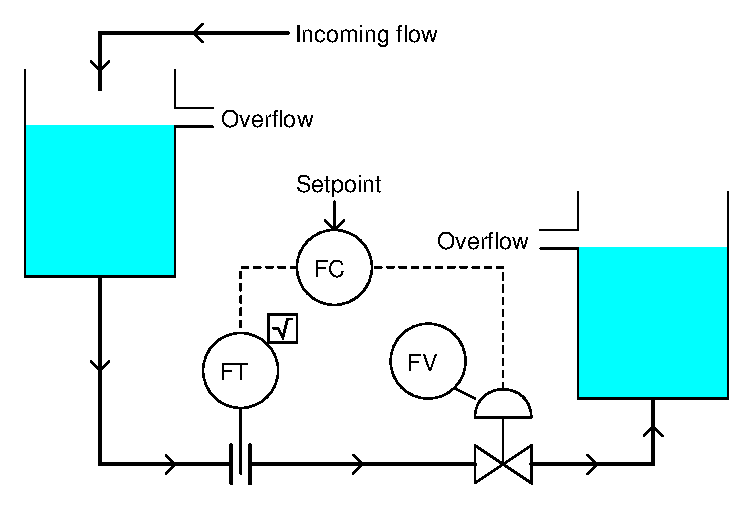
\includegraphics[width=15.5cm]{i01458x01.eps}$$

Siden hver beholder har nivået regulert av et overløpsrør, vil nivåtrykket i bunnen av hver være konstant. Dette betyr at differansetrykket over ventilen også vil være konstant.

\vskip 10pt

Anta nå at overløpsrøret i den høyere beholderen flyttes til en lavere plassering, slik at regulert nivå i den beholderen reduseres, og dermed også nivåtrykket i bunnen:

$$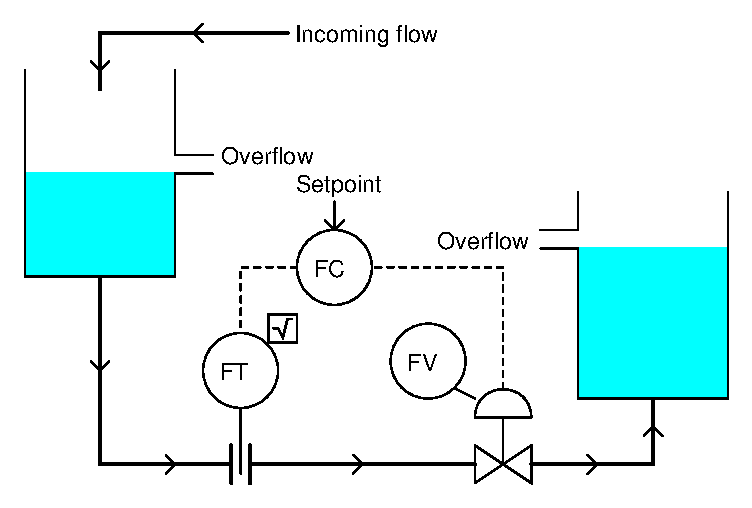
\includegraphics[width=15.5cm]{i01458x02.eps}$$
 
Denne endringen i nivåtrykk vil selvsagt redusere differansetrykket over ventilen. Hvordan påvirker dette prosessgain i forhold til strømningsregulering? Med andre ord: vil strømningsraten bli mer eller mindre følsom for endringer i ventilposisjon når trykkfallet over ventilen reduseres?

\vskip 10pt

Hva skjer med prosessgain hvis vi deretter bytter reguleringsventilen med en som har større $C_v$-verdi (større åpning for væskestrøm når den er helt åpen)?

\vskip 10pt

Til slutt: Hva skjer med prosessgain hvis vi rekalibrerer strømningstransmitteren til et mindre spenn (for eksempel fra 0-120 GPM til 0-75 GPM)?

\underbar{file i01458}
%(END_QUESTION)





%(BEGIN_ANSWER)

Redusert differansetrykk over ventilen vil gi mindre strømning når ventilen står helt åpen. Strømningsraten vil selvsagt fortsatt være null når ventilen er helt stengt. Dette betyr at det regulerbare strømnings{\it området} blir mindre når trykkfallet over ventilen reduseres.

Med et mindre regulerbart strømningsområde vil strømningen ikke endre seg like mye som før for samme endring i ventilposisjon. Det vil si at prosessvariabelen i dette reguleringssystemet blir mindre følsom for endringer i ventilposisjon enn tidligere. Med andre ord står vi overfor {\it redusert} prosessgain.

\vskip 10pt

Med en større ventil vil prosessgain {\it øke}, fordi samme endring i ventilposisjon gir større endringer i strømningsrate når ventilen har større størrelse.

Teknisk sett er ventilgain (forholdet mellom ventilkoeffisient, C$_{v}$, og posisjonsendring) en separat variabel fra prosessgain (forholdet mellom strømningsrate og ventilkoeffisient), og dette er igjen separat fra sensorgain (forholdet mellom transmitterutgang i prosent og strømningsrate). Her brukes likevel begrepet ``prosessgain'' om følsomheten til hele reguleringssystemet unntatt regulatoren (prosessbeholdere og rør, reguleringsventil og strømningstransmitter).

\vskip 10pt

Med en strømningstransmitter med mindre måleområde vil prosessgain {\it øke}, fordi samme ventilposisjonsendringer nå gir større {\it prosentvise} endringer i transmitterutgangen.

%(END_ANSWER)





%(BEGIN_NOTES)


%INDEX% Control, proportional: process gain

%(END_NOTES)

